\documentclass[expologarit]{subfiles}
\begin{document}
\begin{center}
\color{violet} \kml សិក្សាអនុគមន៍ទម្រង់ $y=f(x)=\frac{ax^2+bx+c}{px^2+qx+r}$
\end{center}
\begin{center}
\color{violet} {\kml លំហាត់ទី១}
\end{center}

 $f$ ជាអនុគមន៍កំណត់លើ $\mathrm{I}=\mathbb{R}-\{-2,2\}$ ដោយ $f(x)=\frac{2x^2}{x^2-4}$ ។
\begin{enumerate}[k]
\item សិក្សាលីមីតនៃ $f$ ត្រង់ $-\infty,\ -2,\ 2 $ និង $+\infty$ ។ \\
 ទាញរកសមីការអាស៊ីមតូតដេក និង អាស៊ីមតូតឈរនៃក្រាបតាងអនុគមន៍ $f$ ។
\item សិក្សាអថេរភាព និង សង់តារាងអថេរភាពនៃ $f$ ។
\item សង់នៅក្នុងតម្រុយអរតូណរម៉ាល់ $\left(o,\overrightarrow{i},\overrightarrow{j}\right)$ ក្រាបតាង $f$ ។
\end{enumerate}

\begin{center}
\color{violet} \kml ដំណោះស្រាយ
\end{center}

\begin{enumerate}[k]
\item សិក្សាលីមីតនៃ $f$ ត្រង់ $-\infty,\ -2,\ 2 $ និង $+\infty$ 
\begin{flalign*}
& \lim_{x\to -\infty}f(x)=\lim_{x\to -\infty}\frac{2x^2}{x^2-4}=\lim_{x\to -\infty}\frac{2x^2}{x^2\left(1-\dfrac{4}{x^2}\right)}=\frac{2}{1-0}=2 &\\
&  \text{ដូចនេះ}\ \fbox{$\lim_{x\to -\infty}f(x)=2$}&\\[0.25cm]
&\lim_{x\to -2}f(x)=\lim_{x\to -2}\frac{2x^2}{x^2-4}=\pm \infty \quad \text{ដូចនេះ}\ \fbox{$\lim_{x\to -2}f(x)=\pm \infty $}\\[0.25cm]
&\lim_{x\to 2}f(x)=\lim_{x\to 2}\frac{2x^2}{x^2-4}=\pm \infty \quad \ \ \  \text{ដូចនេះ}\ \fbox{$\lim_{x\to 2}f(x)=\pm \infty $}\\[0.25cm]
& \lim_{x\to +\infty}f(x)=\lim_{x\to +\infty}\frac{2x^2}{x^2-4}=\lim_{x\to +\infty}\frac{2x^2}{x^2\left(1-\dfrac{4}{x^2}\right)}=\frac{2}{1-0}=2\\
& \text{ដូចនេះ}\ \fbox{$\lim_{x\to +\infty}f(x)=2$}&
\end{flalign*}
\newpage 
 ទាញរកសមីការអាស៊ីមតូតដេក និង អាស៊ីមតូតឈរនៃក្រាបតាង $f$ 
 \begin{itemize}
 \item ដោយ $\lim_{x\to \pm \infty}f(x)=2$ \quad  ដូចនេះ\ \fbox{ បន្ទាត់ $y=2$ ជាអាស៊ីមតូតដេក}\\
 \item ដោយ $ \lim_{x\to -2}f(x)=\pm \infty $\ ; $ \lim_{x\to 2}f(x)=\pm \infty $ \\[0.25cm] ដូចនេះ\ \fbox{ បន្ទាត់ $x=-2$ និង $x=-2$ ជាអាស៊ីមតូតឈរ}
 \end{itemize}
\item សិក្សាអថេរភាព និង សង់តារាងអថេរភាពនៃ $f$ 
\begin{itemize}
\item ដេរីវេ 
\begin{flalign*}
 f'(x)&=\left(\frac{2x^2}{x^2-4}\right)'=\frac{\left(2x^2\right)'\left(x^2-4\right)-\left(x^2-4\right)'\left(2x^2\right)}{\left(x^2-4\right)^2}
 =\frac{4x\left(x^2-4\right)-2x\left(2x^2\right)}{\left(x^2-4\right)^2}&\\
 &=\frac{4x^3-16x-4x^3}{\left(x^2-4\right)}=\frac{-16x}{\left(x^2-4\right) }&\\[0.25cm]
 f'(x)&=0\quad \Leftrightarrow\ -16x=0\quad \Rightarrow\ x=0
\end{flalign*}

\item តារាសញ្ញាដេរីវេ $f'(x)$
\\[0.2cm]
\begin{tikzpicture}[scale=0.5]
   \tkzTabInit{$x$ / 1.5 , $f'(x)$ / 2}{$\ \ -\infty$ , $-2$,$0$,$2$, $+\infty\ \ $}
   \tkzTabLine{, +, d, + ,z,-, d,- }
\end{tikzpicture}
\item $f'(x)>0$ ឬ អនុគមន៍ $f$ កើន នៅពេល $x\in\left(-\infty ,-2\right)\cup\left(-2,0\right)$ 
\item $f'(x)<0$ ឬ អនុគមន៍ $f$ ចុះ នៅពេល $x\in\left(0 ,2\right)\cup\left(2,+\infty\right)$ 
\item ត្រង់ $x=0;\ f'(x)=0$ ហើយប្តូរសញ្ញាពី $-$ ទៅ $+$ \\[0.25cm]
គេបាន $f$ មានអតិបរមាធៀបមួយ គឺ $f(0)=\frac{2(0)^2}{0^2-4}=0$
\newpage 
\item តារាងអថេរភាពនៃ $f$\\[0.2cm]
\begin{tikzpicture}
   \tkzTabInit[lw=1,lgt=1,espcl=1.5]{$x$ / 0.75 , $f'(x)$ / 1, $f(x)$/2}{$\ \ -\infty$ , $-2$,$0$,$2$, $+\infty\ \ $}
   \tkzTabLine{, +, d, + ,z,-, d,- }
   \tkzTabVar{-/ $2$,  +D-/ $+\infty$ /$-\infty$, +/ $0$ , -D+/$-\infty$/$+\infty$, -/ $2$}
\end{tikzpicture}
\end{itemize}
\item សង់នៅក្នុងតម្រុយអរតូណរម៉ាល់ $\left(o,\overrightarrow{i},\overrightarrow{j}\right)$ ក្រាបតាង $f$ 
\end{enumerate}
\begin{center}
\definecolor{qqwuqq}{rgb}{0.,0.39215686274509803,0.}
\begin{tikzpicture}[x=0.75cm, y=0.75cm]
\begin{axis}[
x=0.75cm,y=0.75cm,
axis lines=middle,
xlabel=$x$,ylabel=$y$,
xmin=-7.5,
xmax=7.5,
ymin=-6,
ymax=7.5,
xtick={-7,-6,-5,...,8},
ytick={-5,-4,-3,...,8},]

\draw[line width=1.pt,color=qqwuqq,smooth,samples=100,domain=-9:9] plot(\x,{(2.0*(\x)^(2.0))/((\x)^(2.0)-4.0)});
\addplot[domain=-9:9]  {2}; 
\draw(2,0)--(2,-3.5)node[sloped,very near end, above]{$x=2$}; \draw(-2,0)--(-2,-3.5)node[sloped,very near end ,below]{$x=-2$};
\draw(6,1.6)node{$y=2$};
\draw(3,7)node{$(c)$};
\end{axis}
\end{tikzpicture}
\end{center}

\newpage
\begin{center}
\color{violet} \kml លំហាតទី២
\end{center}

អនុគមន៍ $f$ កំណត់ចំពោះ $x\neq -2,\ \ x\neq 2$ ដោយ $y=f(x)=\frac{x^2}{4-x^2}$ និងមានក្រាប $C$ ។ 
		\begin{enumerate}[m]
		\item គណនា $\lim_{x\to -2}f(x),\ \lim_{x\to 2}f(x)$ និង $\lim_{x\to \pm \infty}f(x)$ ។\\
			 ទាញរកសមីការអាស៊ីមតូតឈរ និង អាស៊ីមតូតដេកនៃក្រាប $C$ ។
		\item សិក្សាសញ្ញានៃដេរីវេ $f'(x)$ និងសង់តារាងអថេរភាពនៃ $f$ ។
		\item គណនា $f(-3)$ និង $f(3)$ ហើយសង់ក្រាប $C$ នៃអនុគមន៍ $f$ ។
		\end{enumerate}
	\begin{center}
	\color{violet} \kml ដំណោះស្រាយ
\end{center}		
			\begin{enumerate}[m]
		\item គណនា $\lim_{x\to -2}f(x),\ \lim_{x\to 2}f(x)$ និង $\lim_{x\to \pm \infty}f(x)$ \\[0.25cm]
		ដោយ $y=f(x)=\frac{x^2}{4-x^2}$ គេបាន
		\begin{flalign*}
		\lim_{x\to -2}f(x)&=\lim_{x\to -2}\frac{x^2}{4-x^2}=\pm\infty\quad \fbox{$\lim_{x\to -2}f(x)=\pm\infty$}&\\
		\lim_{x\to 2}f(x)&=\lim_{x\to 2}\frac{x^2}{4-x^2}=\pm\infty\quad\  \fbox{$\lim_{x\to 2}f(x)=\pm\infty$} \\
				\lim_{x\to \pm\infty}f(x)&=\lim_{x\to \pm \infty}\frac{x^2}{4-x^2}=-1 \quad \fbox{$\lim_{x\to \pm\infty}f(x)=-1$}
\end{flalign*}				

		 ទាញរកសមីការអាស៊ីមតូតឈរ និង អាស៊ីមតូតដេកនៃក្រាប $C$
		 \begin{itemize}
		 \item ដោយ $\lim_{x\to -2}f(x)=\pm\infty$ ដូចនេះ \fbox{បន្ទាត់ $x=-2$ ជាអាស៊ីមតូតឈរ}
		 \item $\lim_{x\to 2}f(x)=\pm\infty$ ដូចនេះ \fbox{បន្ទាត់ $x=2$ ជាអាស៊ីមតូតឈរ}
		 	 \item ដោយ $\lim_{x\to \pm\infty}f(x)=-1$ ដូចនេះ \fbox{បន្ទាត់ $y=-1$ ជាអាស៊ីមតូតដេក}
		 \end{itemize}
		\item សិក្សាសញ្ញានៃដេរីវេ $f'(x)$ និងសង់តារាងអថេរភាពនៃ $f$ 
		\begin{flalign*}
		f'(x)&=\left(\frac{x^2}{4-x^2}\right)'=\frac{2x\left(4-x^2\right)+2x\left(x^2\right)}{\left(x^2\right)^2}=\frac{8x-2x^3+2x^3}{x^4}=\frac{8x}{x^4}&
		\end{flalign*}
		ដោយ $x^4\geq 0\quad \forall x\in D_f$\quad  គេបាន $f'(x)$ មានសញ្ញាតាមភាគយក $8x$\\
		$f'(x)=0\quad\Leftrightarrow\quad 8x=0\quad\Rightarrow\quad x=0$\\
តារាសញ្ញាដេរីវេ $f'(x)$
\\[0.2cm]
\begin{tikzpicture}
   \tkzTabInit[lw=1,lgt=1,espcl=1.5]{$x$ / 0.75 , $f'(x)$ / 1}{$\ \ -\infty$ , $-2$,$0$,$2$, $+\infty\ \ $}
   \tkzTabLine{, -, d, - ,z,+, d,+ }
\end{tikzpicture}
\begin{itemize}
\item $f'(x)<0$ ឬ អនុគមន៍ $f$ ចុះ ពេល $x\in\left(-\infty ,-2\right)\cup\left(-2,0\right)$
\item $f'(x)>0$ ឬ អនុគមន៍ $f$ កើន ពេល $x\in\left(0,2\right)\cup\left(2,+\infty\right)$
\item  ត្រង់ $x=0;\ f'(x)=0$ ហើយប្តូរសញ្ញាពី $-$ ទៅ $+$ \\[0.25cm]
គេបាន $f$ មានអប្បបរមាធៀបមួយ គឺ $f(0)=\frac{(0)^2}{4-0^2}=0$
\end{itemize}
 តារាងអថេរភាពនៃ $f$\\[0.2cm]
\begin{tikzpicture}
   \tkzTabInit[lw=1,lgt=1,espcl=1.5]{$x$ / 0.75 , $f'(x)$ / 1, $f(x)$/1.5}{$\ \ -\infty$ , $-2$,$0$,$2$, $+\infty\ \ $}
   \tkzTabLine{, -, d, - ,z,+, d,+ }
   \tkzTabVar{+/ $-1$,  -D+/ $-\infty$ /$+\infty$, -/ $0$ , +D-/$+\infty$/$-\infty$, +/ $-1$}
\end{tikzpicture}
		\item គណនា $f(-3)$ និង $f(3)$ ហើយសង់ក្រាប $C$ នៃអនុគមន៍ $f$ 
		\begin{itemize}
		\item $f(-3)=\frac{(-3)^2}{4-(-3)^2}=\frac{9}{-5}$\quad \fbox{$f(-3)=-\frac{9}{5}$}\\[0.25cm]
		\item $f(3)=\frac{3^2}{4-3^2}=\frac{9}{-5}$\quad \fbox{$f(3)=-\frac{9}{5}$}
		\end{itemize}
	
		\end{enumerate}

	\begin{center}
\definecolor{qqwuqq}{rgb}{0.,0.39215686274509803,0.}
\begin{tikzpicture}[x=1cm, y=1cm]
\begin{axis}[
x=1cm,y=1cm,
axis lines=middle,
xlabel=$x$,ylabel=$y$,
xmin=-6.5,
xmax=6.5,
ymin=-9,
ymax=8.5,
xtick={-8,-7,...,8},
ytick={-9,-8,...,8},]
\draw[line width=1.pt,color=qqwuqq,smooth,samples=300,domain=-9:9] plot(\x,{((\x)^(2.0))/(-(\x)^(2.0)+4.0)});
\addplot[line width=1.2pt,domain=-9:9]  {-1}; 
\draw(2,0)--(2,-6.5)node[sloped,very near end, below]{$x=2$}; \draw(-2,0)--(-2,-6.5)node[sloped,very near end ,above]{$x=-2$};
\draw(5.5,-0.8)node{$y=-1$};
\draw(1.25,7.75)node{$(C)$};
\draw(0,0)node{$\bullet$};
\draw[dashed](-3,0)--(-3,-1.8)node{$\bullet$}--(0,-1.8);
\draw[dashed](3,0)--(3,-1.8)node{$\bullet$}--(0,-1.8);
\end{axis}
\end{tikzpicture}
\end{center}

\newpage 
\begin{center}
\color{violet} \kml លំហាត់ទី៣
\end{center}
អនុគមន៍ $f$ មួយកំណត់ដោយ $y=f(x)=\frac{2x^2-9x+4}{x^2+x-12}$ មានក្រាបតំណាង $(C)$ ។ 
\begin{enumerate}[k]
\item ចូររកដែនកំណត់នៃអនុគមន៍ $f$ ។
\item ចូរគណនាលីមីត៖ $\lim_{x\to -4}f(x)\ ;\ \lim_{x\to 3}f(x)$ និង $\lim_{x\to \pm\infty}f(x)$ ។
\item កំណត់សមីការអាស៊ីមតូតឈរ និងអាស៊ីមតូតដេកនៃក្រាប$(C)$ ។
\item គណនាដេរីវេនៃអនុគមន៍ $f$ រួចសិក្សាសញ្ញាដេរីវេ។
\item សង់តារាងអថេរភាពនៃអនុគមន៍ $f$ និងសង់ក្រាប$(C)$ ។ 
\end{enumerate}

\begin{center}
\color{violet} \kml ដំណោះស្រាយ
\end{center}

\begin{enumerate}[k]
\item រកដែនកំណត់នៃអនុគមន៍ $f$ 
\\[0.25cm] យើងមាន  $y=f(x)=\frac{2x^2-9x+4}{x^2+x-12}$ \\
ដោយ $f(x)$ មានន័យលុះត្រាតែ $ \begin{aligned}[t]
x^2+x-12\neq 0\quad \Leftrightarrow & (x+4)(x-3)\neq 0  \\
\quad\Rightarrow & \left\{\begin{array}{ll}
x+4\neq 0  \\
x-3\neq 0 
\end{array}\right.  \Rightarrow \left\{\begin{array}{ll}
x\neq -4\\
x\neq 3
\end{array}\right.
\end{aligned}  $
\\
ដូចនេះ \fbox{$D_f=\mathbb{R}-\{-4,3\}$}
\item គណនាលីមីត៖ $\lim_{x\to -4}f(x)\ ;\ \lim_{x\to 3}f(x)$ និង $\lim_{x\to \pm\infty}f(x)$ 
\begin{flalign*}
&\lim_{x\to -4}f(x)=\lim_{x\to -4}\frac{2x^2-9x+4}{x^2+x-12}=\pm \infty &\\
&\lim_{x\to 3}f(x)=\lim_{x\to 3}\frac{2x^2-9x+4}{x^2+x-12}=\pm \infty\\
&\lim_{x\to \pm\infty}f(x)=\lim_{x\to \pm\infty}\frac{2x^2-9x+4}{x^2+x-12}=\lim_{x\to \pm\infty}\frac{x^2\left(2-\frac{9}{x}+\frac{4}{x^2}\right)}{x^2\left(1+\frac{1}{x}-\frac{12}{x^2}\right)}=2
\end{flalign*}
\newpage 
\item កំណត់សមីការអាស៊ីមតូតឈរ និងអាស៊ីមតូតដេកនៃក្រាប$(C)$ 
\\
ដោយ $\lim_{x\to -4}f(x)=\pm\infty$ និង $\lim_{x\to 3}f(x)=\pm\infty$\\[0.25cm]
ដូចនេះ \fbox{បន្ទាត់ $x=-4$ និង $x=3$ ជាអាស៊ីមតូតឈរនៃក្រាប$C$ }\\[0.25cm]
ដោយ $\lim_{x\to \pm\infty}f(x)=2$\quad ដូចនេះ \fbox{បន្ទាត់ $y=2$ ជាអាស៊ីមតូតដេក}
\item គណនាដេរីវេនៃអនុគមន៍ $f$ 
\begin{flalign*}
f'(x)=\left(\frac{2x^2-9x+4}{x^2+x-12}\right)' &=\frac{(4x-9)\left(x^2+x-12\right)-(2x+1)\left(2x^2-9x+4\right)}{\left(x^2+x-12\right)^2} &\\
&=\frac{11x^2-56x+104}{\left(x^2+x-12\right)^2}
\end{flalign*}
ដូចនេះ \fbox{$f'(x)=\frac{11x^2-56x+104}{\left(x^2+x-12\right)^2}$}
\\[0.25cm]
សិក្សាសញ្ញាដេរីវេ\\
$f'(x)=0\Leftrightarrow 11x^2-56x+104=0\quad \Rightarrow \Delta =(-56)^2-4(11)(104)=-1440<0$\\
យើងបាន $f'(x)$ មានសញ្ញាដូចមេគុណ $a$ 
\\[0.2cm]
\begin{tikzpicture}[scale=1]
   \tkzTabInit[lw=1,lgt=1,espcl=1.5]{$x$ / 1 , $f'(x)$ / 1}{$ -\infty$ , $-4$,$3$, $+\infty $}
   \tkzTabLine{, +, d, +, d,+ }
\end{tikzpicture}\\
$f'(x)>0\quad \forall x\in\mathbb{D_f}$ ដូចនេះ អនុគមន៍ $f$ ជាអនុគមន៍កើនលើដែនកំណត់ $D_f$
\item សង់តារាងអថេរភាពនៃអនុគមន៍ $f$ និងសង់ក្រាប$(C)$ \\
 តារាងអថេរភាពនៃ $f$\\[0.2cm]
\begin{tikzpicture}
   \tkzTabInit[lw=1,lgt=1,espcl=2]{$x$ / 0.75 , $f'(x)$ / 1, $f(x)$/1.5}{$ -\infty$ , $-4$,$3$, $+\infty $}
   \tkzTabLine{, +, d, +, d,+ }
   \tkzTabVar{-/$2$,  +D-/ $+\infty$ /$-\infty$ , +D-/$+\infty$/$-\infty$, +/ $2$}
\end{tikzpicture}\\
សង់ក្រាប
\begin{flalign*}
(C)\cap (x'Ox)\Leftrightarrow y=0\quad\Leftrightarrow \quad & 2x^2-9x+4=0 &\\
&\Delta =b^2-4ac=(-9)^2-4(2)(4)=81-32=49 \\
\Rightarrow\quad & x_1=\frac{-b-\sqrt{\Delta}}{2a}=\frac{9-\sqrt{49}}{2(2)}=\frac{1}{2} \\
& x_2=\frac{-b+\sqrt{\Delta}}{2a}=\frac{9+\sqrt{49}}{2(2)}=4
\end{flalign*}
\begin{flalign*}
&(C)\cap (y'Oy) \Leftrightarrow x=0\quad \Rightarrow\quad y=\frac{2(0)^2-9(0)+4}{0^2+0-12}=\frac{4}{-12}=-\frac{1}{3} &\\
&(C)\cap (d):y=2\Leftrightarrow 2=\frac{2x^2-9x+4}{x^2+x-12}\quad  \Rightarrow x=\frac{28}{11}
\end{flalign*}
\begin{itemize}
\item អាស៊ីមតូតឈរ $x=-4, \ x=3$\qquad អាស៊ីមតូតដេក $y=2$
\end{itemize}
\end{enumerate}
\begin{center}
\begin{tikzpicture}[x=1cm,y=1cm]
\begin{axis}[scale=1,
          xmax=10.5,ymax=11.5,
          axis lines=middle,
          xmin=-13.5,ymin=-10.5,          
          xtick={-12,-10,...,10},
          ytick={-12,-10,...,12}  ,
          xlabel=$x$   ,
          ylabel=$y$   ,x=0.5cm, y=0.5cm
          ] 
\addplot[domain=-13:10 ,restrict y to domain=-14:14,line width=1pt,samples=5000,smooth,name path=A,color=red] {(2*x^2-9*x+4)/(x^2+x-12)};
\addplot[domain=-14.5:10,line width=1.5pt,samples=100,smooth] {2}node[sloped, near end,above]{$\qquad\qquad\qquad\qquad\qquad
y=2$};

%\addplot [color=black]coordinates {(-2.5,0)} node[below ]{$x'$};

%\node at(0,-1){$\bullet$};

%\draw[dashed](1,0)--(1,1)--(0,1);

             %\addplot[gray, pattern=north west lines] fill between[of=A and B, soft clip={domain=1:2}];
            

       
        
  
              \draw (0,0)rectangle (0.2,0.2);
           
             \draw[line width=1.5pt] (3,-14)--(3,14)node[sloped, near end,below]{$x=3$};
                          \draw[line width=1.5pt] (-4,-14)--(-4,14)node[sloped, near end,below]{$x=-4$};
            \draw (-6,11) node {$(C)$};
             \draw (0.5,0) node {$\bullet$};
              \draw (0,-0.33) node {$\bullet$};
              \draw[dashed](2.5,0)--(2.5,2)node{$\bullet$};
\end{axis}
\end{tikzpicture}
 \end{center}
\newpage
\begin{center}
\color{violet} \kml លំហាត់ទី៤
\end{center} 
 គេមានអនុគមន៍ $f$ មួយកំណត់ដោយ $y=f(x)=\frac{3x^2-18x+25}{x^2-6x+8}$ មានក្រាបតំណាង$(C)$។
 \begin{enumerate}[k]
 \item រកដែនកំណត់នៃអនុគមន៍$f$។
 \item គណនាលីមីតនៃអនុគមន៍$f$ ត្រង់ $\pm\infty\ ;\ 2$ និង $4$ ។ រួចទាញរកសមីការអាស៊ីមតូតឈរ និងដេក។
 \item ចូរបង្ហាញថា $f'(x)=\frac{-2x+6}{\left(x^2-6x+8\right)^2}$ ចំពោះគ្រប់ $x\in \mathbb{R}-\{2,4\} $។
 \item សិក្សាសញ្ញាដេរីវេ$f'(x)$ និងសង់តារាងអថេរភាពនៃអនុគមន៍$f$។
 \item សង់ក្រាប $(C)$។
 \end{enumerate}
 \begin{center}
 \color{violet} \kml ដំណោះស្រាយ
 \end{center}
  \begin{enumerate}[k]
 \item រកដែនកំណត់នៃអនុគមន៍$f$
យើងមាន $y=f(x)=\frac{3x^2-18x+25}{x^2-6x+8}$ \\
$f(x)$ មានន័យលុះត្រាតែ $\begin{aligned}[t]
x^2-6x+8 \neq 0 \Leftrightarrow & \quad (x-2)(x-4)\neq 0 \\
\Leftrightarrow & \left\{\begin{array}{ll}
x-2\neq 0\\
x-4\neq 0
\end{array}\right.\Rightarrow \left\{\begin{array}{ll}
x\neq 2\\
x\neq 4
\end{array}\right.
\end{aligned}  $
 \\
 ដូចនេះ \fbox{$D_f=\mathbb{R}-\{2,4\}$}
 \item គណនាលីមីតនៃអនុគមន៍$f$ ត្រង់ $\pm\infty\ ;\ 2$ និង $4$ 
\begin{flalign*}
&\lim_{x\to \pm\infty}f(x)=\lim_{x\to \pm\infty}\frac{3x^2-18x+25}{x^2-6x+8} =\lim_{x\to \pm\infty}\frac{x^2\left(3-\frac{18}{x}+\frac{25}{x^2}\right)}{x^2\left(1-\frac{6}{x}+\frac{8}{x^2}\right)}=3&\\
&\lim_{x\to 2}f(x)=\lim_{x\to 2}\frac{3x^2-18x+25}{x^2-6x+8}=\pm\infty\\
&\lim_{x\to 4}f(x)=\lim_{x\to 4}\frac{3x^2-18x+25}{x^2-6x+8}=\pm\infty
\end{flalign*} 
 ទាញរកសមីការអាស៊ីមតូតឈរ និងដេក\\
 ដោយ $\lim_{x\to 2}f(x)=\pm\infty\ ;\ \lim_{x\to 4}f(x)=\pm\infty$\\[0.25cm]
 ដូចេនះ \fbox{បន្ទាត់ $x=2$;\ $x=4$ ជាអាស៊ីមតតូតឈរ}\\[0.25cm]
 ដោយ $\lim_{x\to \pm\infty}f(x)=3$ \\[0.25cm]
 ដូចនេះ \fbox{បន្ទាត់ $y=3$ ជាអាស៊ីមតូតដេក}
 \item បង្ហាញថា $f'(x)=\frac{-2x+6}{\left(x^2-6x+8\right)^2}$ ចំពោះគ្រប់ $x\in \mathbb{R}-\{2,4\} $
 \begin{flalign*}
 f'(x)&=\left(\frac{3x^2-18x+25}{x^2-6x+8}\right)'&\\[0.25cm]
 &=\frac{(6x-18)\left(x^2-6x+8\right)-\left(2x-6\right)\left(3x^2-18x+25\right)}{\left(x^2-6x+8\right)^2}&\\
 &= \frac{-2x+6}{\left(x^2-6x+8\right)^2}
 \end{flalign*}
 ដូចនេះ \fbox{$f'(x)=\frac{-2x+6}{\left(x^2-6x+8\right)^2}$}
 \item សិក្សាសញ្ញាដេរីវេ$f'(x)$
\begin{align*}
f'(x)=0\Leftrightarrow -2x+6=0\quad\Rightarrow x=3 &&
\end{align*} 
តារាសញ្ញាដេរីវេ $f'(x)$
\\[0.2cm]
\begin{tikzpicture}
   \tkzTabInit[lw=1,lgt=1,espcl=1.5]{$x$ / 0.75 , $f'(x)$ / 1}{$\ \ -\infty$ , $2$,$3$,$4$, $+\infty\ \ $}
   \tkzTabLine{, +, d, + ,z,-, d,- }
\end{tikzpicture}
\begin{itemize}
\item $f'(x)<0$ ឬ អនុគមន៍ $f$ ចុះ ពេល $x\in\left(3 ,4\right)\cup\left(4,+\infty\right)$
\item $f'(x)>0$ ឬ អនុគមន៍ $f$ កើន ពេល $x\in\left(-\infty,2\right)\cup\left(2,3\right)$
\item  ត្រង់ $x=3;\ f'(x)=0$ ហើយប្តូរសញ្ញាពី $+$ ទៅ $-$ \\[0.25cm]
គេបាន $f$ មានអតិបរមាធៀបមួយ គឺ $f(3)=\frac{3(3)^2-18(3)+25}{3^2-6(3)+8}=2$
\end{itemize}
\newpage 
 សង់តារាងអថេរភាពនៃអនុគមន៍$f$\\[0.25cm]
 \begin{tikzpicture}
   \tkzTabInit[lw=1,lgt=1,espcl=1.5]{$x$ / 0.75 , $f'(x)$ / 1, $f(x)$/1.5}{$\ \ -\infty$ , $2$,$3$,$4$, $+\infty\ \ $}
   \tkzTabLine{, +, d, + ,z,-, d,- }
   \tkzTabVar{-/ $3$,  +D-/ $+\infty$ /$-\infty$, +/ $2$ , -D+/$-\infty$/$+\infty$, -/ $3$}
\end{tikzpicture}
 \item សង់ក្រាប $(C)$
 \begin{flalign*}
& (C)\cap (x'ox)\Leftrightarrow y=0 \Leftrightarrow 3x^2-18x+25=0 \Rightarrow x_1=\frac{9-\sqrt{6}}{3}\ ;\ x_2=\frac{9+\sqrt{6}}{3} &\\
 & (C)\cap (y'oy)\Leftrightarrow x=0\Rightarrow y=\frac{3(0)^2-18(0)+25}{0^2-6(0)+8}=\frac{25}{8}
 \end{flalign*}
 \end{enumerate}
 \begin{center}
\begin{tikzpicture}[x=1cm,y=1cm]
\begin{axis}[scale=1,
          xmax=8.5,ymax=7.5,
          axis lines=middle,
          xmin=-3.5,ymin=-3.5,          
          xtick={-11,-10,...,10},
          ytick={-11,-10,...,12}  ,
          xlabel=$x$   ,
          ylabel=$y$   ,x=1cm, y=1cm
          ] 
\addplot[domain=-13:13 ,restrict y to domain=-14:14,line width=1pt,samples=1000,smooth,name path=A,color=red] {(3*x^2-18*x+25)/(x^2-6*x+8)};
\addplot[domain=-14.5:13,samples=100,smooth] {3}node[sloped, near end,below]{$\qquad\qquad\qquad\qquad\qquad
y=3$};

%\addplot [color=black]coordinates {(-2.5,0)} node[below ]{$x'$};

%\node at(0,-1){$\bullet$};

%\draw[dashed](1,0)--(1,1)--(0,1);

             %\addplot[gray, pattern=north west lines] fill between[of=A and B, soft clip={domain=1:2}];
           
              \draw (0,0)rectangle (0.2,0.2);
           
             \draw[line width=1.5pt] (2,-14)--(2,14)node[sloped, near end,below]{$x=2$};
                          \draw[line width=1.5pt] (4,-14)--(4,14)node[sloped, near end,above]{$x=4$};
            \draw (3.5,-3) node {$(C)$};
             \draw[dashed] (3,0)--(3,2) node {$\bullet$}--(0,2);
              \draw (0,3.1) node {$\bullet$};
              \draw (2.2,0) node {$\bullet$};
              \draw (3.8,0) node {$\bullet$};
\end{axis}
\end{tikzpicture}
 \end{center}
 \newpage
 \begin{center}
\color{violet}  \kml លំហាត់ទី៥
 \end{center}
 គេឲ្យអនុគមន៍ $f$មួយ កំណត់ដោយ $y=f(x)=\frac{x^2+2x}{x^2+4}$ មានក្រាបតំណាង$(C)$ ។
 \begin{enumerate}[k]
 \item រកដែនកំណត់នៃអនុគមន៍$f$។ 
 \item រកសមីការអាស៊ីមតូតដេកនៃក្រាប$(C)$។
 \item សិក្សាអថិរភាព និងសង់តារាងអថិរភាពនៃអនុគមន៍$f$ ។
 \item សង់ក្រាប $(C)$ ក្នុងតម្រុយ$\left(O,\overrightarrow{i},\overrightarrow{j}\right)$។
 \end{enumerate}
 \begin{center}
 \kml
 \color{violet} ដំណោះស្រាយ
 \end{center}
  \begin{enumerate}[k]
 \item រកដែនកំណត់នៃអនុគមន៍$f$
យើងមាន  $y=f(x)=\frac{x^2+2x}{x^2+4}$\\
$f(x)$ មានន័យលុះត្រាតែ $x^2+4\neq 0 $  ដោយ $x^2+4\neq 0\quad\forall x\in\mathbb{R}$\\
ដូចនេះ \fbox{$D_f=\mathbb{R}$}
  
 \item រកសមីការអាស៊ីមតូតដេកនៃក្រាប$(C)$
\\
ដោយ $\lim_{x\to\pm \infty}f(x)=\lim_{x\to \pm\infty}\frac{x^2+2x}{x^2+4}=1$ 
 \\
 ដូចនេះ \fbox{បន្ទាត់ $y=1$ ជាអាស៊ីមតូតដេកនៃក្រាប$(C)$}
 \item សិក្សាអថិរភាព និងសង់តារាងអថិរភាពនៃអនុគមន៍$f$\\
 ដេរីវេ$f'(x)$
 \begin{flalign*}
 f'(x)&=\left(\frac{x^2+2x}{x^2+4}\right)'&\\
 		&=\frac{(2x+2)\left(x^2+4\right)-(2x)\left(x^2+2x\right)}{\left(x^2+4\right)^2}\\
 		&=\frac{2x^3+8x+2x^2+8-2x^3-4x^2}{\left(x^2+4\right)^2}\\
 		&=\frac{-2x^2+8x+8}{\left(x^2+4\right)^2}
 \end{flalign*}
 \newpage 
 \begin{flalign*}
 f'(x)=0\Leftrightarrow\quad & -2x^2+8x+8=0 &\\
 												& \Delta =b^2-4ac=8^2-4(-2)(8)=64+64=128\\
 	\Rightarrow\quad  & x_1=\frac{-b-\sqrt{\Delta}}{2a}=\frac{-8-\sqrt{128}}{2(-2)}=\frac{-8-8\sqrt{2}}{-4}=2+2\sqrt{2} 		\\
& 	x_2=\frac{-b+\sqrt{\Delta}}{2a}=\frac{-8+\sqrt{128}}{2(-2)}=\frac{-8+8\sqrt{2}}{-4}=2-2\sqrt{2} 		
 \end{flalign*}
 តារាសញ្ញាដេរីវេ $f'(x)$
\\[0.2cm]
\begin{tikzpicture}
   \tkzTabInit[lw=1,lgt=1.5,espcl=2]{$x$ / 0.75 , $f'(x)$ / 1}{$ -\infty$ , $2-2\sqrt{2}$,$2+2\sqrt{2}$, $+\infty $}
   \tkzTabLine{, -, z, + , z,- }
\end{tikzpicture}
\begin{itemize}
\item $f'(x)<0$ ឬ អនុគមន៍ $f$ ចុះ នៅពេល $x\in\left(-\infty ,2-2\sqrt{2}\right)\cup\left(2+2\sqrt{2},+\infty\right)$
\item $f'(x)>0$ ឬ អនុគមន៍ $f$ កើន នៅពេល $x\in\left(2-2\sqrt{2},\ 2+2\sqrt{2}\right)$
\end{itemize}
បរមាធៀប៖
\begin{itemize}
\item ត្រង់ $x=2-2\sqrt{2},\ f'(x)=0$ ហើយប្តូរសញ្ញាពី$-$ ទៅ $+$ យើងបាន $f$ មានអប្បបរមាធៀបមួយគឺ $\begin{aligned}[t]
f(2-2\sqrt{2})=\frac{\left(2-2\sqrt{2}\right)^2+2\left(2-2\sqrt{2}\right)}{\left(2-2\sqrt{2}\right)^2+4}
&=\frac{4-8\sqrt{2}+8+4-4\sqrt{2}}{4-8\sqrt{2}+8+4}&\\
&=\frac{16-12\sqrt{2}}{16-8\sqrt{2}} =\frac{4-3\sqrt{2}}{4-2\sqrt{2}}\times\frac{4+2\sqrt{2}}{4+2\sqrt{2}}\\
&=\frac{16+8\sqrt{2}-12\sqrt{2}-12}{16-8}\\
&=\frac{4-4\sqrt{2}}{8}=\frac{1-\sqrt{2}}{2}
\end{aligned} $\\
\item ត្រង់ $x=2+2\sqrt{2},\ f'(x)=0$ ហើយប្តូរសញ្ញាពី$+$ ទៅ $-$ យើងបាន $f$ មានអតិបរមាធៀបមួយគឺ 
\begin{align*}
f(2+2\sqrt{2})=\frac{\left(2+2\sqrt{2}\right)^2+2\left(2+2\sqrt{2}\right)}{\left(2+2\sqrt{2}\right)^2+4}
&=\frac{4+8\sqrt{2}+8+4+4\sqrt{2}}{4+8\sqrt{2}+8+4}&\\
&=\frac{16+12\sqrt{2}}{16+8\sqrt{2}} =\frac{4+3\sqrt{2}}{4+2\sqrt{2}}\times\frac{4-2\sqrt{2}}{4-2\sqrt{2}}\\
&=\frac{16-8\sqrt{2}+12\sqrt{2}-12}{16-8}\\
&=\frac{4+4\sqrt{2}}{8}=\frac{1+\sqrt{2}}{2}
\end{align*}
\item តារាងអថេរភាពនៃអនុគមន៍$f$
\\[0.25cm]
 \begin{tikzpicture}
   \tkzTabInit[lw=1,lgt=1.5,espcl=2]{$x$ / 0.75 , $f'(x)$ / 1,$f(x)$/2.5}{$ -\infty$ , $2-2\sqrt{2}$,$2+2\sqrt{2}$, $+\infty $}
   \tkzTabLine{, -, z, + , z,- }
   \tkzTabVar{+/ $1$, -/ $\tfrac{1-\sqrt{2}}{2}$ , +/ $\tfrac{1+\sqrt{2}}{2}$, -/ $1$}
\end{tikzpicture}
\end{itemize}
 \item សង់ក្រាប $(C)$ ក្នុងតម្រុយ$\left(O,\overrightarrow{i},\overrightarrow{j}\right)$
\begin{itemize}
\item $(C)\cap (x'ox)\Leftrightarrow y=0\Leftrightarrow x^2+2x=0\Leftrightarrow (x)(x+2)=0\quad \Rightarrow x=0,x=-2$
\item $(C)\cap (y'oy)\Leftrightarrow x=0\Rightarrow y=\frac{0^2+2(0)}{0^2+4}=0$
\item $(C)\cap (d):y=1\Leftrightarrow 1=\frac{x^2+2x}{x^2+4}\Leftrightarrow x^2+4=x^2+2x\quad \Rightarrow x=2$
\end{itemize} 
 
 \end{enumerate}
  \begin{center}
\begin{tikzpicture}[x=1cm,y=1cm]
\begin{axis}[scale=1,
          xmax=5.5,ymax=2.5,
          axis lines=middle,
          xmin=-7.5,ymin=-1.5,          
          xtick={-11,-10,...,10},
          ytick={-11,-10,...,12}  ,
          xlabel=$x$   ,
          ylabel=$y$   ,x=1cm, y=1cm
          ] 
\addplot[domain=-13:13 ,restrict y to domain=-14:14,line width=1pt,samples=1000,smooth,name path=A,color=red] {(x^2+2*x)/(x^2+4)};
\addplot[domain=5.5:-7.5,samples=100,smooth] {1}node[sloped, near end,above]{$y=1$};

%\addplot [color=black]coordinates {(-2.5,0)} node[below ]{$x'$};

%\node at(0,-1){$\bullet$};

%\draw[dashed](1,0)--(1,1)--(0,1);

             %\addplot[gray, pattern=north west lines] fill between[of=A and B, soft clip={domain=1:2}];
           
              \draw (0,0)rectangle (0.2,0.2);
            \draw (-7,0.35) node {$(C)$};
             \draw[dashed] (4.8,0)--(4.8,1.2) node {$\bullet$}--(0,1.2);
              \draw[dashed] (-0.8,0)--(-0.8,-0.2) node {$\bullet$}--(0,-0.2);
              \draw (0,0) node {$\bullet$};
              \draw (2,1) node {$\bullet$};
                 \draw (-2,0) node {$\bullet$};
            
\end{axis}
\end{tikzpicture}
 \end{center}
 \newpage
 \begin{center}
\color{violet}  \kml លំហាត់ទី៦
 \end{center}
គេមានអនុគមន៍$f$មួយ កំណត់ដោយលើ $\mathbb{R}-\{-2\}$ ដែល $y=f(x)=\frac{x^2-1}{(x+2)^2}$។\\ តាង$(C)$ ជាក្រាបតំណាងនៃអនុគមន៍$f$។  
 \begin{enumerate}[k]
 \item គណនា $\lim_{x\to -2}f(x)\ ;\ \lim_{x\to \pm\infty}f(x)$។ រួចទាញរកសមីការអាស៊ីមតូតទាំងអស់ដែលមាន។
 \item គណនាដេរីវេ$f'(x)$ រួចបង្ហាញថាអនុគមន៍$f$ មានតម្លៃអប្បបរមាធៀបមួយស្មើ $-\frac{1}{3}$ ត្រង់ $x=-\frac{1}{2}$។
 \item សង់តារាងអថិរភាព រួចសង់ក្រាប$(C)$។
 \end{enumerate}
 \begin{center}
\color{violet}  \kml ដំណោះស្រាយ
 \end{center}
  \begin{enumerate}[k]
 \item គណនា $\lim_{x\to -2}f(x)\ ;\ \lim_{x\to \pm\infty}f(x)$
 \begin{flalign*}
 &\lim_{x\to -2}f(x)=\lim_{x\to -2}\frac{x^2-1}{(x+2)^2}=+\infty &\\
 &\lim_{x\to \pm\infty}f(x)=\lim_{x\to \pm\infty}\frac{x^2\left(1-\frac{1}{x^2}\right)}{x^2\left(1+\frac{2}{x}\right)^2}=1
 \end{flalign*}
  ទាញរកសមីការអាស៊ីមតូតទាំងអស់ដែលមាន
  \\
  ដោយ $\lim_{x\to -2}f(x)=+\infty$\quad\ ដូចនេះ \fbox{បន្ទាត់$x=-2$ជាអាស៊ីមតូតឈរនៃក្រាប$(C)$}\\[0.25cm]
   ដោយ $\lim_{x\to \pm\infty}f(x)=1$\quad ដូចនេះ \fbox{បន្ទាត់$y=1$ជាអាស៊ីមតូតដេកនៃក្រាប$(C)$}
 \item គណនាដេរីវេ$f'(x)$ 
\begin{flalign*}
f'(x)=\left(\frac{x^2-1}{(x+2)^2}\right)'&=\frac{2x(x+2)^2-2(x+2)\left(x^2-1\right)}{(x+2)^4}&\\
&=\frac{2x\left( x^2+4x+4\right)-2x^3+2x-4x^2+4}{(x+2)^4}\\
&=\frac{2x^3+8x^2+8x-2x^3+2x-4x^2+4}{(x+2)^4}\\
&=\frac{4x^2+10x+4}{(x+2)^4}
\end{flalign*} 
ដូចនេះ \fbox{$f'(x)=\frac{4x^2+10x+4}{(x+2)^4}$}\\[0.25cm]
 បង្ហាញថាអនុគមន៍$f$ មានតម្លៃអប្បបរមាធៀបមួយស្មើ $-\frac{1}{3}$ ត្រង់ $x=-\frac{1}{2}$
\begin{flalign*}
f'(x)=0\Leftrightarrow\quad 4x^2+10x+4=0\Leftrightarrow\quad & (4x+2)(x+2)=0&\\
\Rightarrow\quad & \left[\begin{array}{ll}
4x+2=0\\
x+2=0
\end{array}\right.\Rightarrow\quad \left[\begin{array}{l}
x=-\frac{1}{2}\\
x=-2
\end{array}\right.
\end{flalign*}
 តារាងសញ្ញា$f'(x)$ 
 \\[0.2cm]
\begin{tikzpicture}
   \tkzTabInit[lw=1,lgt=1.5,espcl=2]{$x$ / 1 , $f'(x)$ / 1}{$ -\infty$ , $-2$,$-\frac{1}{2}$, $+\infty $}
   \tkzTabLine{, +, d, - , z,+ }
\end{tikzpicture}
\\
ត្រង់ $x=-\frac{1}{2};\ f'(x)=0$ ហើយប្តូរសញ្ញាពី$-$ទៅ$+$ យើងបាន$f$ មានអប្បបរមាធៀបមួយគឺ
\begin{flalign*}
f\left(-\frac{1}{2}\right)=\frac{\left(-\frac{1}{2}\right)^2-1}{\left(\left(-\frac{1}{2}\right)+2\right)^2}&=\frac{\frac{1}{4}-1}{\left(\frac{3}{2}\right)^2}=\frac{-\frac{3}{4}}{\frac{9}{4}}=-\frac{3}{4}\times\frac{4}{9}=-\frac{1}{3}&
\end{flalign*}
ដូចនេះ \fbox{អនុគមន៍$f$ មានតម្លៃអប្បបរមាធៀបមួយស្មើ $-\frac{1}{3}$ ត្រង់ $x=-\frac{1}{2}$}
 \item តារាងអថិរភាពនៃអនុគមន៍$f$
  \\[0.2cm]
\begin{tikzpicture}
   \tkzTabInit[lw=1,lgt=1.5,espcl=2]{$x$ / 1 , $f'(x)$ / 1,$f(x)$/2}{$ -\infty$ , $-2$,$-\frac{1}{2}$, $+\infty $}
   \tkzTabLine{, +, d, - , z,+ }
      \tkzTabVar{-/ $1$, +D+/ $+\infty$/ \ $+\infty$ , -/ $-\tfrac{1}{3}$, +/ $1$}
\end{tikzpicture}
 \newpage 
 សង់ក្រាប$(C)$
 \begin{flalign*}
 &(C)\cap (x'ox)\Leftrightarrow y=0\quad\Leftrightarrow\quad x^2-1=0\quad\Rightarrow\ x=\pm 1 &\\
 &(C)\cap (y'oy)\Leftrightarrow x=0\quad\Rightarrow\quad y=\frac{0^2-1}{(0+2)^2}=\frac{-1}{4}
 \end{flalign*}
$ \begin{aligned}[t]
  (C)\cap (d):y=1\quad \Leftrightarrow\quad & 1=\frac{x^2-1}{(x+2)^2}\\
  \Leftrightarrow\quad & (x+2)^2=x^2-1\\
  \Leftrightarrow\quad & x^2+4x+4=x^2-1\quad \Rightarrow x=-\frac{5}{4}
 \end{aligned}$
 \end{enumerate}
 \begin{center}
\begin{tikzpicture}[x=1cm,y=1cm]
\begin{axis}[scale=1,
          xmax=4.5,ymax=8.5,
          axis lines=middle,
          xmin=-8,ymin=-2.5,          
          xtick={-12,-11,...,10},
          ytick={-12,-11,...,12}  ,
          xlabel=$x$   ,
          ylabel=$y$   ,x=1cm, y=1cm
          ] 
\addplot[domain=-13:10 ,restrict y to domain=-14:14,line width=1pt,samples=1000,smooth,name path=A,color=red] {(x^2-1)/(x+2)^2};
\addplot[domain=-14.5:10,line width=1.5pt,samples=100,smooth] {1}node[sloped, near end,above]{$\qquad\qquad\qquad\qquad\qquad
y=1$};

%\addplot [color=black]coordinates {(-2.5,0)} node[below ]{$x'$};

%\node at(0,-1){$\bullet$};

%\draw[dashed](1,0)--(1,1)--(0,1);

             %\addplot[gray, pattern=north west lines] fill between[of=A and B, soft clip={domain=1:2}];
            

       
        
  
              \draw (0,0)rectangle (0.2,0.2);
           
  
                          \draw[line width=1.5pt] (-2,-14)--(-2,14)node[sloped, near end,above]{$x=-2$};
            \draw (-4,8) node {$(C)$};
             \draw [dashed](-0.5,0)--(-0.5,-0.33) node {$\bullet$}--(0,-0.33);
              \draw (0,-0.25) node {$\bullet$};
               \draw[dashed](-1.25,0)-- (-1.25,1) node {$\bullet$};
\end{axis}
\end{tikzpicture}
 \end{center}
 \newpage
 \begin{center}
\color{violet}  \kml លំហាត់ទី៧
 \end{center}
 អនុគមន៍$f$ មួយកំណត់ដោយ $y=f(x)=\frac{-x^2-2x+3}{x^2+3x+2}$ មានក្រាបតំណាង$(C)$។
 \begin{enumerate}[k]
 \item រកដែនកំណត់នៃអនុគមន៍ $f$ ។
 \item សិក្សាលីមីតនៃអនុគមន៍ $f$ ត្រង់ $-1,\ -2$ និង $\pm\infty$។ ទាញរកអាស៊ីមតូតដេក និងអាស៊ីមតូតឈរទាំងពីរ។
 \item ចំពោះគ្រប់$x\in\mathbb{R}-\{-1,-2\}$ ចូរគណនាដេរីវេ$f'(x)$។
 \item សិក្សាសញ្ញាដេរីវេ $f'(x)$ រួចសង់តារាងអថិរភាពនៃអនុគមន៍ $f$ ។
 \item ចូរសង់ក្រាប $(C)$ ក្នុងតម្រុយ $(O,\overrightarrow{i},\overrightarrow{j})$
 \end{enumerate}
 \begin{center}
\color{violet}  \kml ដំណោះស្រាយ
 \end{center}
  \begin{enumerate}[k]
 \item រកដែនកំណត់នៃអនុគមន៍ $f$ \\
យើងមាន $y=f(x)=\frac{-x^2-2x+3}{x^2+3x+2}$\\[0.25cm]
$f(x)$ មានន័យលុះត្រាតែ $x^2+3x+2\neq 0 \Leftrightarrow\quad (x+1)(x+2)\neq 0\quad \Rightarrow\ x\neq -1;\ x\neq -2 $\\[0.25cm]
ដូចនេះ \fbox{$D_f=\mathbb{R}-\{-1,-2\}$}
 \item សិក្សាលីមីតនៃអនុគមន៍ $f$ ត្រង់ $-1,\ -2$ និង $\pm\infty$
\begin{flalign*}
&\lim_{x\to -1}f(x)=\lim_{x\to -1}\frac{-x^2-2x+3}{x^2+3x+2}=\pm\infty &\\
&\lim_{x\to -2}f(x)=\lim_{x\to -2}\frac{-x^2-2x+3}{x^2+3x+2}=\pm\infty &\\
&\lim_{x\to \pm\infty}f(x)=\lim_{x\to \pm\infty}\frac{-x^2-2x+3}{x^2+3x+2}= \lim_{x\to \pm\infty}\frac{x^2\left(-1-\frac{2}{x}+\frac{3}{x^2}\right)}{x^2\left(1+\frac{3}{x}+\frac{2}{x^2}\right)}=-1  &
\end{flalign*} 
  ទាញរកអាស៊ីមតូតដេក និងអាស៊ីមតូតឈរទាំងពីរ\\
  ដោយ $\lim_{x\to \pm\infty}f(x)=-1$\quad ដូចនេះ \fbox{បន្ទាត់ $y=-1$ ជាអាស៊ីមតូតដេកនៃក្រាប$(C)$}
  \\[0.25cm]
  ដោយ $\lim_{x\to -1}f(x)=\pm\infty\ ;\lim_{x\to -2}f(x)=\pm\infty$\\[0.25cm]
  ដូចនេះ \fbox{បន្ទាត់ $x=-1$ និង $x=-2$ ជាអាស៊ីមតូតឈរនៃក្រាប$(C)$ }
  \newpage 
 \item ចំពោះគ្រប់$x\in\mathbb{R}-\{-1,-2\}$ គណនាដេរីវេ$f'(x)$
\begin{flalign*}
f'(x)=\left(\frac{-x^2-2x+3}{x^2+3x+2}\right)'&=\frac{(-2x-2)\left(x^2+3x+2\right)-(2x+3)\left(-x^2-2x+3\right)}{\left(x^2+3x+2\right)^2}&\\
&=\frac{-x^2-10x-13}{\left(x^2+3x+2\right)^2}
\end{flalign*} 
 ដូចនេះ \fbox{$f'(x)=\frac{-x^2-10x-13}{\left(x^2+3x+2\right)^2}$}
 \item សិក្សាសញ្ញាដេរីវេ $f'(x)$
\begin{flalign*}
f'(x)=0\quad\Leftrightarrow\quad & -x^2-10x-13=0 &\\
					 & \Delta =b^2-4ac=\left(-10\right)^2-4(-1)(-13)=100-52=48\\
					 \Rightarrow \quad & x_1=\frac{-b-\sqrt{\Delta}}{2a}=\frac{10-\sqrt{48}}{2(-1)}=\frac{10-4\sqrt{3}}{-2}=-5+2\sqrt{3}\\
					 & x_2=\frac{-b+\sqrt{\Delta}}{2a}=\frac{10+\sqrt{48}}{2(-1)}=\frac{10+4\sqrt{3}}{-2}=-5-2\sqrt{3}
\end{flalign*} 
 តារាសញ្ញាដេរីវេ $f'(x)$
\\[0.2cm]
\begin{tikzpicture}
   \tkzTabInit[lw=1,lgt=1.5,espcl=2]{$x$ / 0.75 , $f'(x)$ / 1}{$ -\infty$ , $-5-2\sqrt{3}$,$-2$,$-5+2\sqrt{3}$,$-1$, $+\infty $}
   \tkzTabLine{, -, z,+ ,d, + , z, -, d ,- }
\end{tikzpicture}
\begin{itemize}
\item $f'(x)>0$ ពេល $x\in\left(-5-2\sqrt{3},-2\right)\cup\left(-2,-5+2\sqrt{3}\right)$
\item $f'(x)<0$ ពេល $x\in\left(-\infty ,-5-2\sqrt{3}\right)\cup\left(-5+2\sqrt{3},-1\right)\cup\left(-1,+\infty\right)$
\end{itemize}
បរមាធៀប
\begin{itemize}
\item ត្រង់ $x=-5-2\sqrt{3};\ f'(x)=0$ ហើយប្តូរសញ្ញាពី$-$ទៅ$+$ នោះ $f$ មានអប្បបរមាធៀបមួយគឺ 
\begin{flalign*}
f(-5-2\sqrt{3})&=\frac{-\left(-5-2\sqrt{3}\right)^2-2\left(-5-2\sqrt{3}\right)+3}{\left(-5-2\sqrt{3}\right)^2+3\left(-5-2\sqrt{3}\right)+2}=4\sqrt{3}-8 &
\end{flalign*}
\item ត្រង់ $x=-5+2\sqrt{3};\ f'(x)=0$ ហើយប្តូរសញ្ញាពី$+$ទៅ$-$ នោះ $f$ មានអតិបរមាធៀបមួយគឺ 
\begin{flalign*}
f(-5+2\sqrt{3})&=\frac{-\left(-5+2\sqrt{3}\right)^2-2\left(-5+2\sqrt{3}\right)+3}{\left(-5+2\sqrt{3}\right)^2+3\left(-5+2\sqrt{3}\right)+2}=-4\sqrt{3}-8 &
\end{flalign*}
\end{itemize}
 សង់តារាងអថិរភាពនៃអនុគមន៍ $f$ 
 \\[0.2cm]
\begin{tikzpicture}
   \tkzTabInit[lw=1,lgt=1.5,espcl=2]{$x$ / 0.75 , $f'(x)$ / 1,$f(x)$/2}{$ -\infty$ , $-5-2\sqrt{3}$,$-2$,$-5+2\sqrt{3}$,$-1$, $+\infty $}
   \tkzTabLine{, -, z,+ ,d, + , z, -, d ,- }
    \tkzTabVar{+/ $-1$,-/$4\sqrt{3}-8$ ,+D-/ $+\infty$/ \ $-\infty$ ,+/$-4\sqrt{3}-8$, -D+/ $-\infty$ / \ $+\infty$, -/ $-1$}
\end{tikzpicture}
 
 \item សង់ក្រាប $(C)$ ក្នុងតម្រុយ $(O,\overrightarrow{i},\overrightarrow{j})$
\begin{flalign*}
(C)\cap (x'ox)\Leftrightarrow y=0\quad\Leftrightarrow\quad & -x^2-2x+3=0 \Leftrightarrow (-x+1)(x+3)=0 &\\
\Rightarrow\quad &\left[\begin{array}{ll}
-x+1=0\\
x+3=0
\end{array}\right.\Rightarrow \quad\left[\begin{array}{ll}
x=1\\
x=-3
\end{array}\right.
\end{flalign*} 
 \begin{flalign*}
 &(C)\cap (y'oy)\Leftrightarrow x=0\quad\Rightarrow\quad y=\frac{-0^2-2(0)+3}{0^2+3(0)+2}=\frac{3}{2}&
 \end{flalign*}
  \begin{flalign*}
 (C)\cap (d):y=-1\quad\Leftrightarrow\quad  -1=\frac{-x^2-2x+3}{x^2+3x+2}\Leftrightarrow & -x^2-3x-2=-x^2-2x+3 &\\
 \Rightarrow & -x=5 \\
 \Rightarrow & x=-5
 \end{flalign*}
 \end{enumerate}
 \begin{center}
\begin{tikzpicture}[x=1cm,y=1cm]
\begin{axis}[scale=1,
          xmax=3.5,ymax=2.5,
          axis lines=middle,
          xmin=-10.5,ymin=-16.5,          
          xtick={-12,-11,...,10},
          ytick={-16,-15,...,12}  ,
          xlabel=$x$   ,
          ylabel=$y$   ,x=0.75cm, y=1cm
          ] 
\addplot[domain=-13:10 ,restrict y to domain=-19:14,line width=1pt,samples=1000,smooth,name path=A,color=red] {(-1*x^2-2*x+3)/(x^2+3*x+2)};
\addplot[domain=-14.5:3.5,line width=1.5pt,samples=100,smooth] {-1}node[sloped, near end,above]{$y=-1$};

%\addplot [color=black]coordinates {(-2.5,0)} node[below ]{$x'$};

%\node at(0,-1){$\bullet$};

%\draw[dashed](1,0)--(1,1)--(0,1);

             %\addplot[gray, pattern=north west lines] fill between[of=A and B, soft clip={domain=1:2}];
            

       
        
  
              \draw (0,0)rectangle (0.2,0.2);
           
             \draw[line width=1.5pt] (-1,-19)--(-1,14)node[sloped, near end,below]{$x=3$};
                          \draw[line width=1.5pt] (-2,-19)--(-2,14)node[sloped, near end,below]{$x=-4$};
            \draw (-3,2) node {$(C)$};
             \draw (1,0) node {$\bullet$};
              \draw (-3,0) node {$\bullet$};
              \draw (0,1.5) node {$\bullet$};
              \draw[dashed] (-1.55,0)--(-1.55,-14.9)node{$\bullet$}--(0,-14.9);
                \draw[dashed] (-8.46,0)--(-8.46,-1.07)node{$\bullet$}--(0,-1.07);
               \draw[dashed] (-5,0)--(-5,-1)node{$\bullet$}--(0,-1);
\end{axis}
\end{tikzpicture}
 \end{center}
 \newpage 
\subfile{function2-8}
\newpage
\subfile{function2-9}
\newpage 
\subfile{function2-10}
\end{document}